\section{Synthetic Detectors and the Grid}
\label{app:grid}
\begin{figure}[t]
\centering
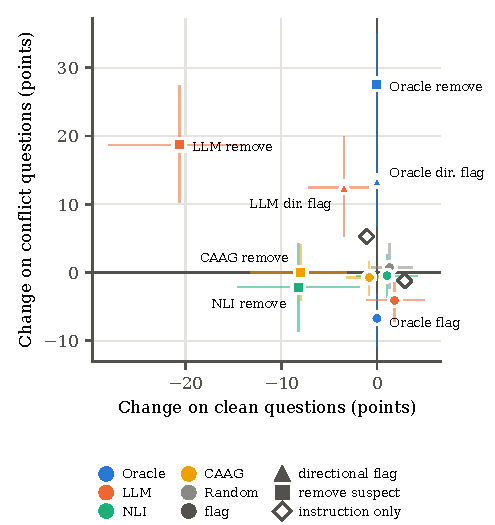
\includegraphics[width=\columnwidth]{generated/fig_tradeoff.pdf}
\caption{Change in one-way strict accuracy on RAMDocs conflict questions (y) against clean questions (x), relative to
no flags (gpt-4o-mini, default skeleton, confirmatory split, 95\% CIs). Colour: detector; shape: format. The oracle
sits on the y-axis because it never flags a clean question. Without direction, removal deletes the second passage of
each pair.}
\label{fig:tradeoff}
\end{figure}

\begin{figure*}[t]
\centering
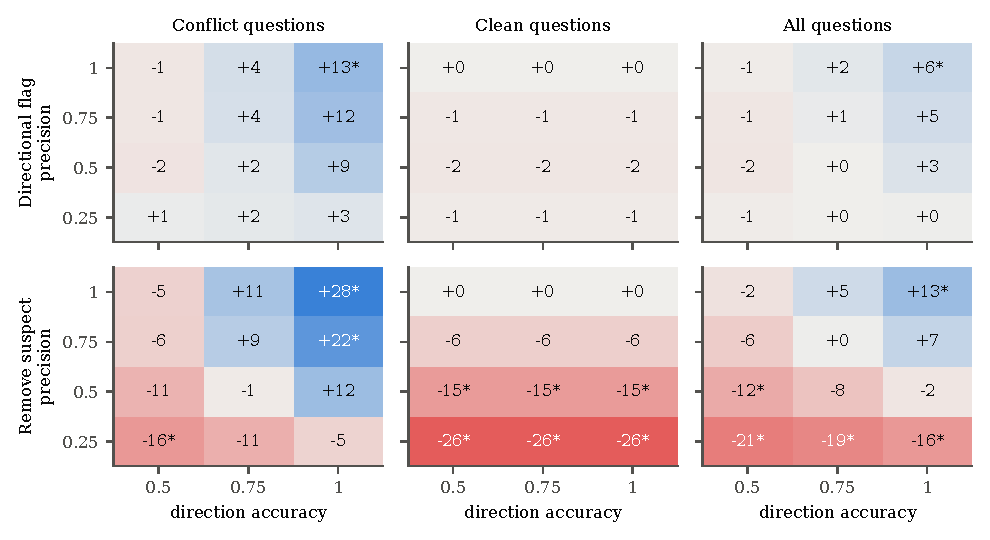
\includegraphics[width=\textwidth]{generated/fig_grid.pdf}
\caption{Synthetic detectors at recall 1: change in one-way strict accuracy (points) against no flags, by pair
precision (rows) and direction accuracy (columns), for the directional flag (top) and removal (bottom). $^*$:
significant after Holm correction over the 36 cells of that mode and subset. Clean questions only see false flags,
so their rows do not vary with direction accuracy.}
\label{fig:grid}
\end{figure*}

Figure~\ref{fig:grid} replaces the oracle with synthetic detectors of known quality. Two thresholds appear. First,
\emph{direction accuracy}: at a direction accuracy of 0.5 or 0.75, no cell gains significantly on all questions in
either format. Only perfect direction does (directional flag \gDirOneDOneAll, removal \gRemOneDOneAll\ points at
perfect precision). Second, \emph{precision}, but mainly for removal. On clean questions a cell's prompt does not depend
on direction accuracy, so the false-flag cells reduce to \hFourRemN\ distinct comparisons per format. Removal is
significantly harmful in \hFourRemHarm\ of them, the directional flag in \hFourDirHarm\ (H4a): false flags make the
model delete correct passages, which costs clean questions \agRemHalfDOneClean\ points at precision 0.5 and
\agRemQuDOneClean\ at 0.25, while synthetic false directional flags cost at most two points. The harm tracks the
share of clean questions that lose a correct document (Spearman $\rho=\hFourRho$ over \hFourRhoCells\ distinct
cells, 95\% CI \hFourRhoCI\ from a question-level bootstrap; H4b). Removal hurt clean questions significantly more
than the directional flag in \hFourRemWorse\ of \hFourMatched\ matched cells (H4c; we set no threshold, so we report
the count). Removal is the more powerful and the more fragile interface: its best cell gains twice the directional
flag's on all questions, but below precision 0.75 it is the only format that does net harm.


\paragraph{Does the grid predict real detectors?}

If the grid only described synthetic detectors, it would be of limited use. Figure~\ref{fig:placement} (Appendix~\ref{app:extra}) tests
whether it predicts real ones (H6). As pre-registered, we bootstrap the whole prediction (cell effects, every detector's
location and the interpolation) over questions, and ask whether the actual effect falls inside the 95\% interval.
Locating detectors by what they do to documents (the share of conflict questions whose misinformation is marked, and
the share of questions that have a correct document marked) puts \hSixDocIn\ of \hSixN\ effects inside; locating them
by pair precision, recall and direction accuracy puts \hSixPairIn\ inside. Document-level errors are smaller on
average (\hSixDocMae\ vs.\ \hSixPairMae\ points), but the paired difference, \hSixMaeDiff\ \hSixMaeDiffCI\ (exact
sign-flip $p=\hSixMaeP$), is not significant over \hSixN\ cases. Both spaces miss the same case, the LLM detector's
removal gain on conflict questions: one correctly directed pair is enough to remove a misinformation document, so the
detector removes the misinformation on \misGoneLlm\% of conflict questions despite its low pair recall. We chose the
document-level axes after seeing the LLM detector on the pilot split. The grid is a useful first estimate of a
detector's effect, but with three detectors we cannot claim that one summary predicts better than the other.

